Beim Start der App sieht man das Logo der App als Splash-Screen (Abbildung \ref{fig:splashundmenu}). Nach dem Laden wird man von der Home-Seite begrüsst. Streift man mit dem Finger von links nach rechts oder klickt auf den Menu-Sandwich, öffnet sich ein Side-Menü. Das Side-Menü hat oben wieder das Logo und 2 Texte darunter ("`Magic 2 Brain"' und "`Your MTG learning companion"'). Darunter befinden sich 7 Buttons mit den Texten: "`Home"', "`Search"', "`Set Browser"', "`Quick Learn"', "`Favorites"', "`Recently Learned"' und "`Share"' (Abbildung \ref{fig:splashundmenu}).

\begin{figure}[htbp] 
  \centering
     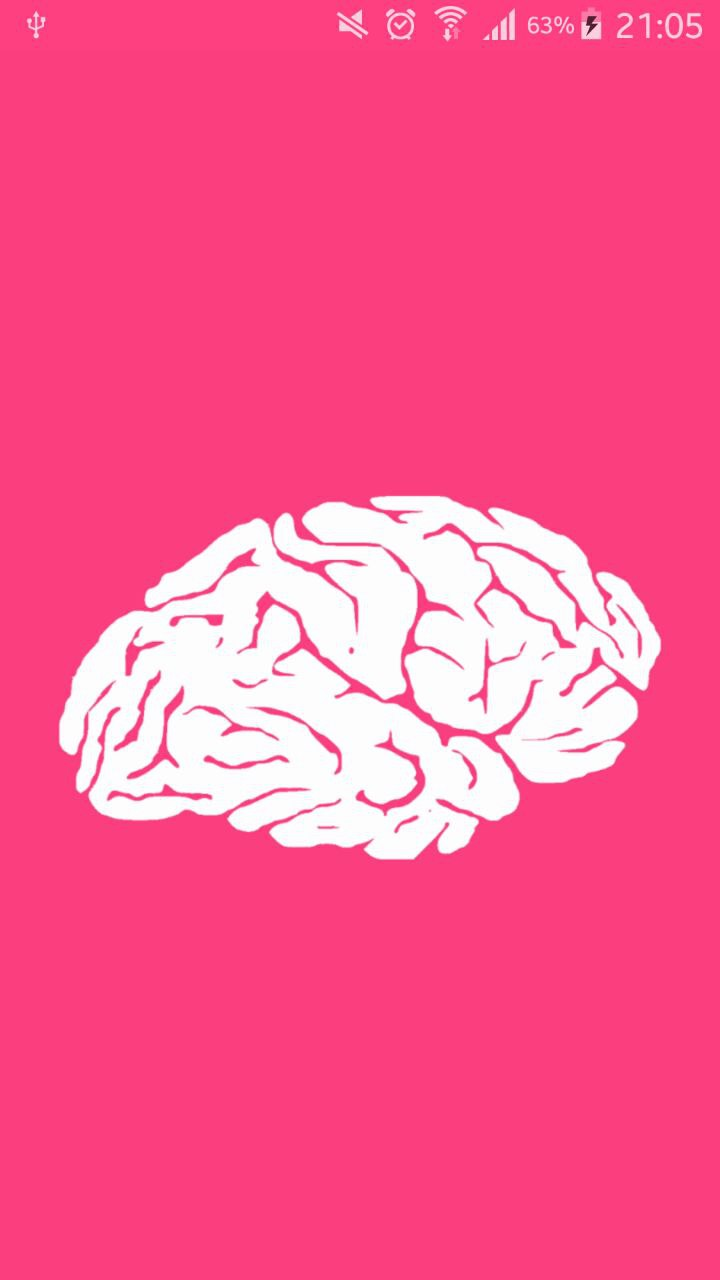
\includegraphics[width=0.3\textwidth]{startup.jpg}
     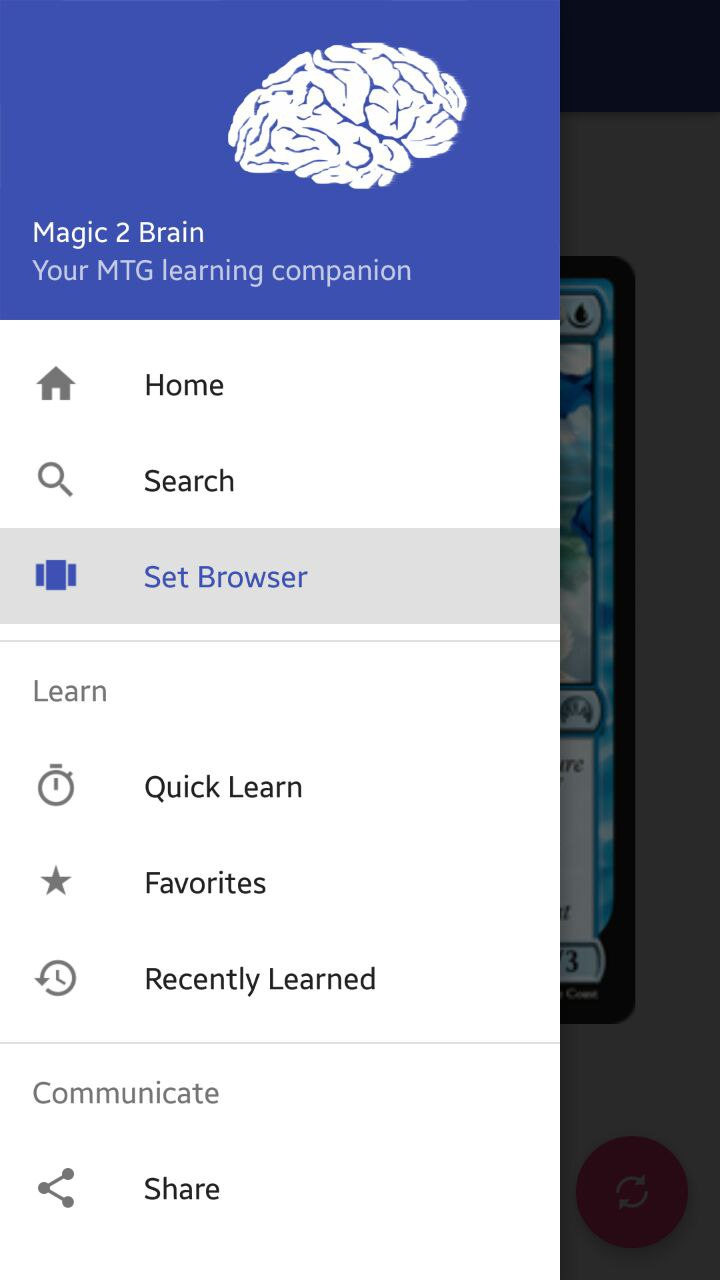
\includegraphics[width=0.3\textwidth]{sidemenu.jpg}
  \caption{Links: Der Splash-Screen, Rechts: Das Menü}
  \label{fig:splashundmenu}
\end{figure}

\subsection{Home}
Der Home-Screen ist simpel aufgebaut. Zuoberst steht "`Magic2Brain"' und darunter "`Random Card"'. Unter diesem Text ist eine zufällige Karte abgebildet. Mit einem Klick auf die Karte lässt die sich vergrössern. Ganz unten rechts ist ein runder Knopf. Dieser ersetzt bei einem Klick die Karte mit einer anderen zufälligen Karte. (Abbildung \ref{fig:homemenu}).

\begin{figure}[htbp] 
  \centering
     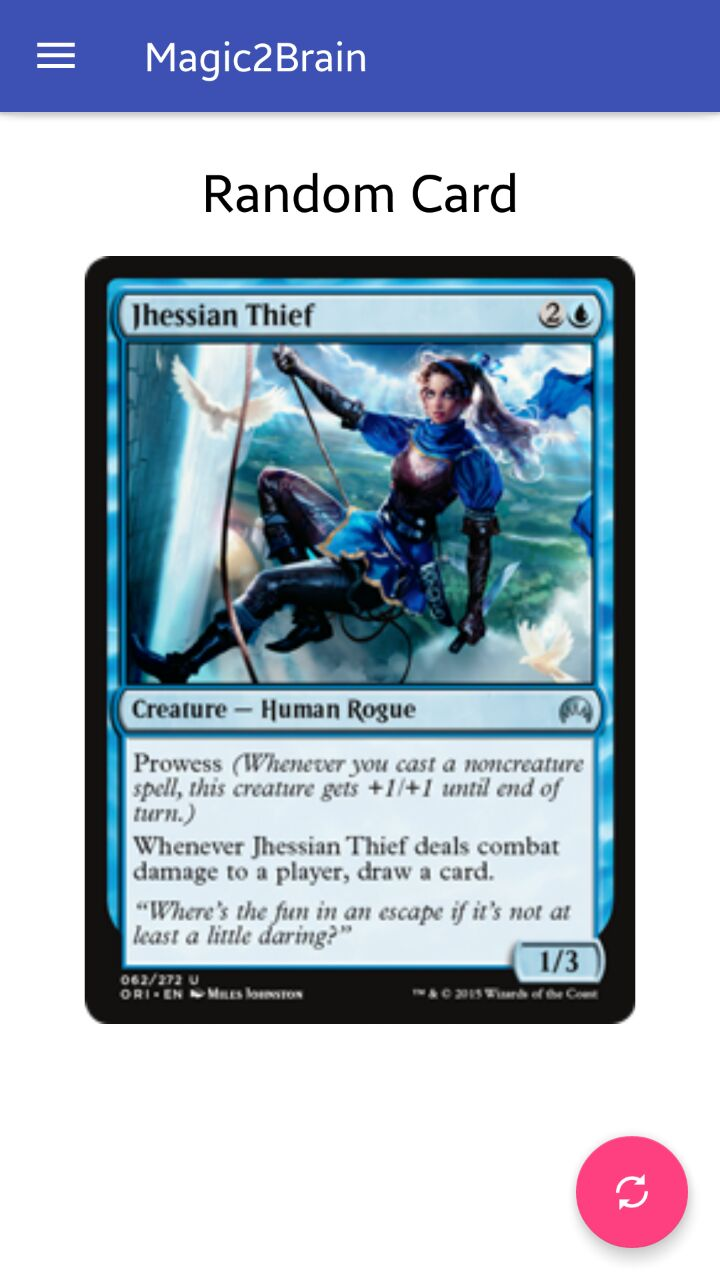
\includegraphics[width=0.3\textwidth]{home.jpg}
  \caption{Der Home-Screen}
  \label{fig:homemenu}
\end{figure}

\subsection{Search}
Klickt man auf "`Search"' kann man auswählen, ob man nach Karten oder Sets suchen möchte. Wählt man einen aus, kommt man zu einer Ansicht mit einem Textfeld und einer Liste darunter. Tippt man etwas in das Textfeld ein, ändert sich die Liste und zeigt nur die Ergebnisse der Suche an.

\subsection{Set Browser}
Der Set-Browser zeigt alle Sets in einer Liste an (Abbildung \ref{fig:setbrowser}). Klick man auf ein Set, kommt man zu einer weiteren Ansicht mit einer Liste. Diese Liste beinhaltet alle Karten vom ausgewählten Set. Klickt man auf eine Karte erhält man einen genaueren Blick auf die Karte. Bild, Text, Manakosten und der Name der Karte werden angezeigt (Abbildung \ref{fig:setbrowser}). Zudem hat man einen Knopf mit einem Herzen drauf. Klickt man diesen, wird die Karte zu den Favoriten hinzugefügt.

\begin{figure}[htbp] 
  \centering
     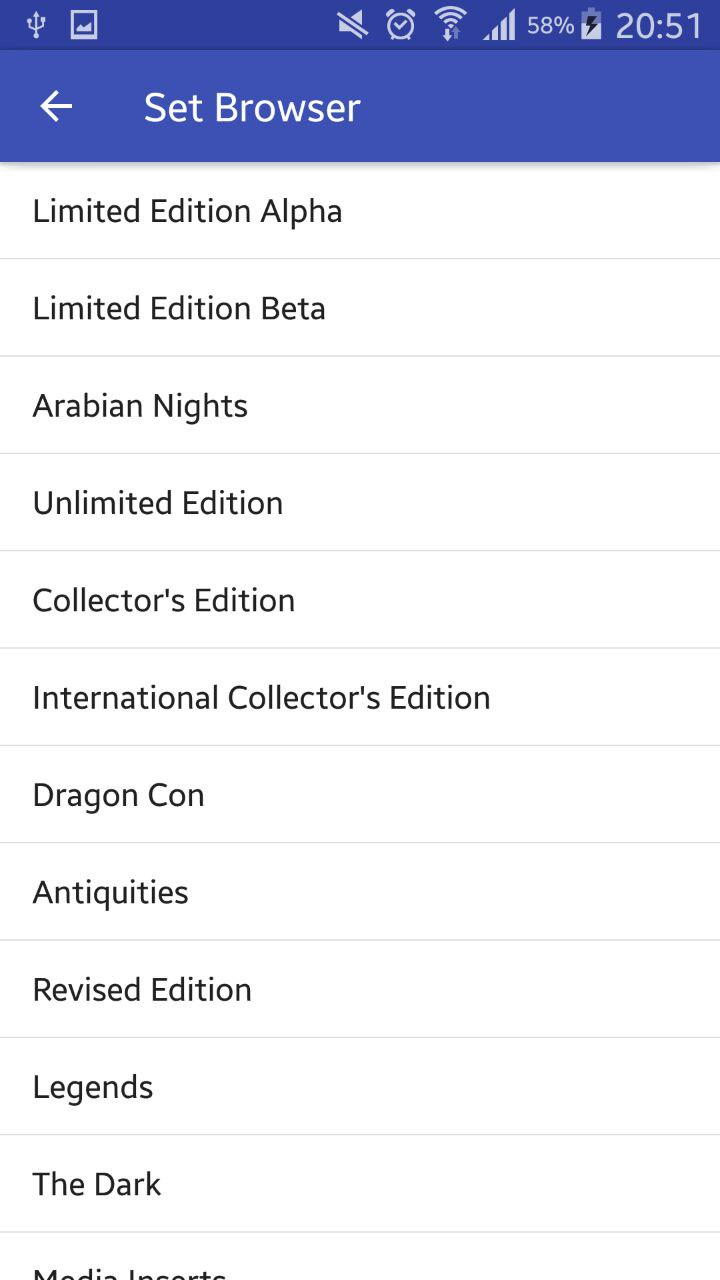
\includegraphics[width=0.3\textwidth]{setbrowser.jpg}
      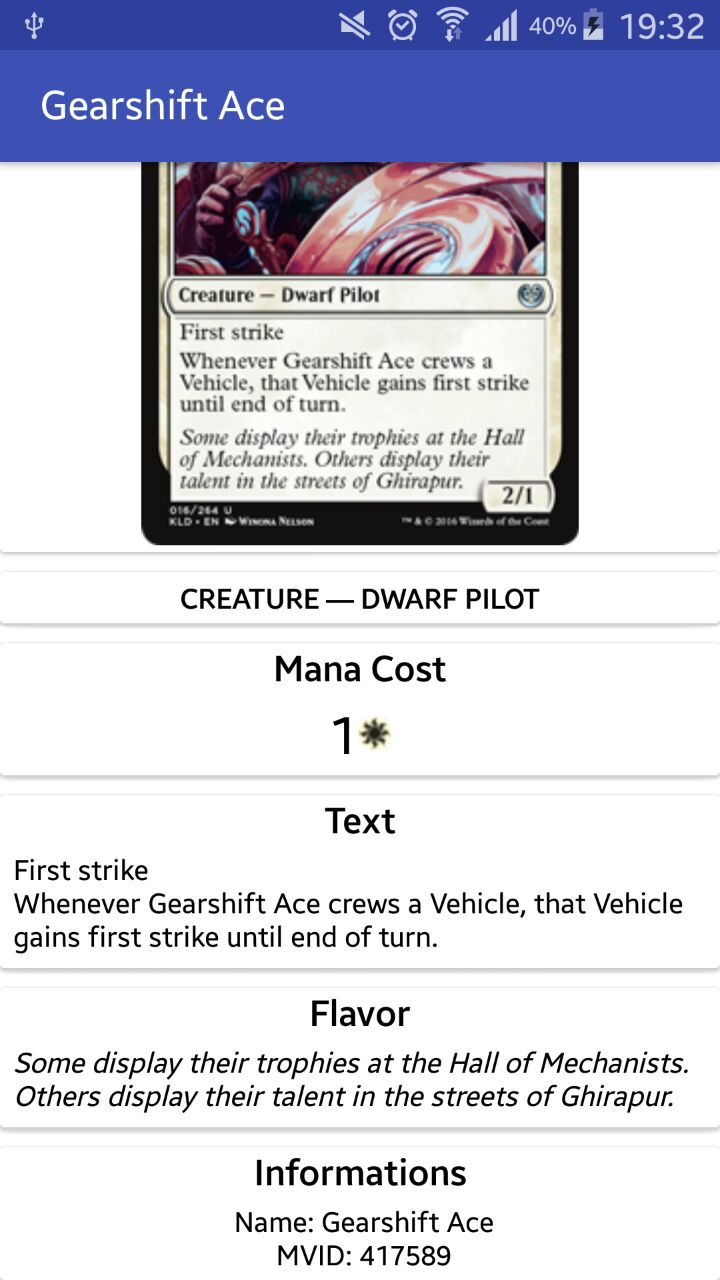
\includegraphics[width=0.3\textwidth]{cardview.jpg}
  \caption{Links: Der Set-Browser, Rechts: Die Karten-Ansicht}
  \label{fig:setbrowser}
\end{figure}

\subsection{Quick Learn}
"`Quick Learn"' startet eine Abfrage mit dem aktuellsten Set. In diesem Fall ist es Kaladesh. (Abbildung \ref{fig:queryview}).

\begin{figure}[htbp] 
  \centering
     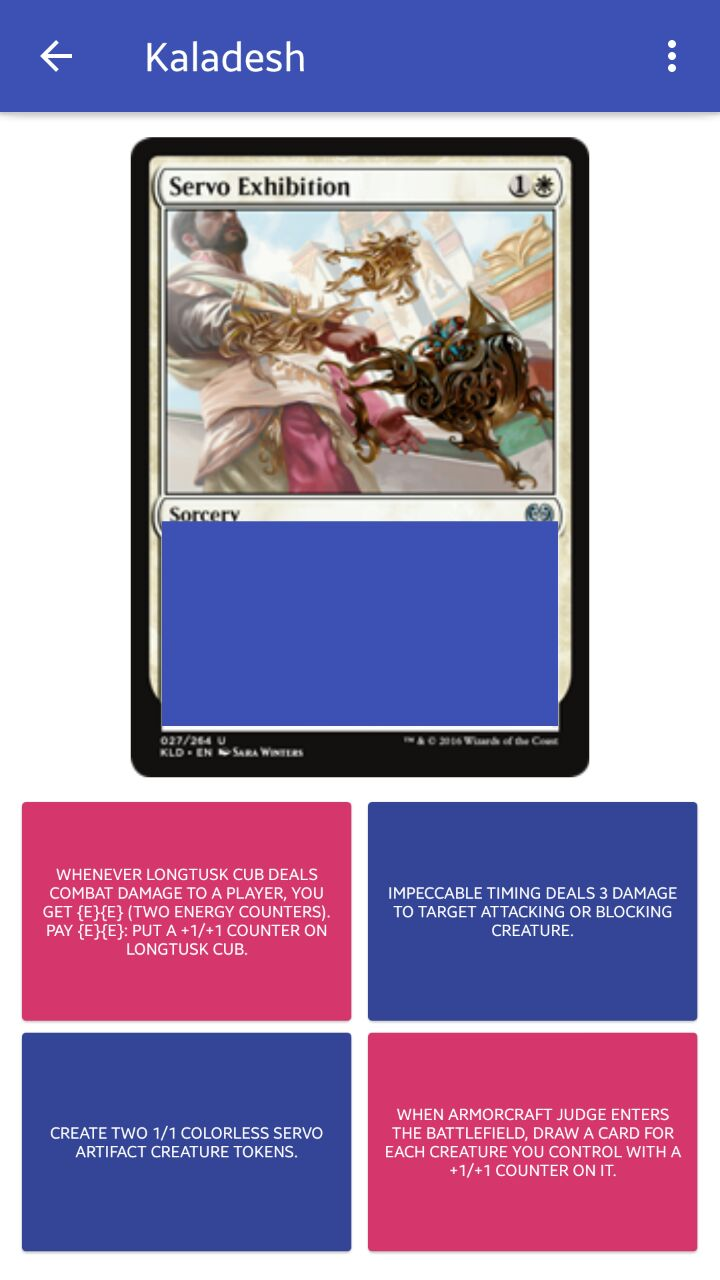
\includegraphics[width=0.3\textwidth]{query.jpg}
  \caption{Die Abfrage eines Sets}
  \label{fig:queryview}
\end{figure}

\subsection{Favorites}
Klickt man auf Favoriten, werden alle Favoriten in einer Liste angezeigt.

\subsection{Recently Learned}
"`Recently Learned"' zeigt die letzten 10 gelernten Sets in einer Liste an.

\subsection{Share}
Klickt man auf diesen Knopf, öffnet sich ein Menü. Bei diesem Menü kann man auswählen über welche App man den Link zu dieser App versenden möchte.